\documentclass[11pt,a4paper]{article}

\usepackage[utf8]{inputenc}
\usepackage[T1]{fontenc}
\usepackage[english]{babel}
\usepackage{geometry}
\geometry{top=2.5cm, bottom=2.5cm, left=2.5cm, right=2.5cm, headheight=14pt}

\usepackage{xcolor}
\definecolor{primaryBlue}{RGB}{11, 60, 93}
\definecolor{steelBlue}{RGB}{31, 110, 165}
\definecolor{skyBlue}{RGB}{225, 238, 248}
\definecolor{mintGreen}{RGB}{46, 125, 50}
\definecolor{mintGreenBg}{RGB}{232, 245, 233}
\definecolor{crimsonRed}{RGB}{183, 28, 28}
\definecolor{examAmber}{RGB}{180, 83, 9}
\definecolor{examAmberBg}{RGB}{254, 243, 199}
\definecolor{bodyDark}{RGB}{30, 41, 59}
\definecolor{codeBg}{RGB}{248, 250, 252}
\definecolor{codeFrame}{RGB}{203, 213, 225}

% macOS Dark Terminal Colors
\definecolor{termbg}{RGB}{15, 23, 36}
\definecolor{termframe}{RGB}{24, 34, 52}
\definecolor{termtitlebar}{RGB}{20, 30, 46}
\definecolor{termred}{RGB}{239, 68, 68}
\definecolor{termyellow}{RGB}{245, 158, 11}
\definecolor{termgreen}{RGB}{34, 197, 94}
\definecolor{termtext}{RGB}{241, 245, 249}

\usepackage{amsmath,amssymb,amsfonts}
\usepackage{booktabs}
\usepackage{tabularx}
\usepackage{graphicx}
\usepackage{subcaption}
\usepackage{hyperref}
\hypersetup{
    colorlinks=true,
    linkcolor=steelBlue,
    citecolor=mintGreen,
    urlcolor=steelBlue,
    pdftitle={Laboratory 02: Encoder-Decoder Models and the Attention Mechanism},
    pdfauthor={Politecnico di Torino - LLM Course}
}

\usepackage{fancyhdr}
\pagestyle{fancy}
\fancyhf{}
\fancyhead[L]{\textsf{\footnotesize \textbf{Laboratory 02}: Encoder-Decoder Models and Attention Mechanism}}
\fancyhead[R]{\textsf{\footnotesize Politecnico di Torino}}
\fancyfoot[C]{\thepage}
\renewcommand{\headrulewidth}{0.4pt}
\renewcommand{\footrulewidth}{0.4pt}

\usepackage{listings}
\usepackage{tcolorbox}
\tcbuselibrary{listings,skins,breakable}

\lstdefinestyle{pythonstyle}{
    language=Python,
    basicstyle=\ttfamily\footnotesize\color{bodyDark},
    keywordstyle=\bfseries\color{primaryBlue},
    stringstyle=\color{mintGreen},
    commentstyle=\itshape\color{gray},
    numberstyle=\tiny\color{gray},
    numbers=left,
    numbersep=8pt,
    stepnumber=1,
    tabsize=4,
    showspaces=false,
    showstringspaces=false,
    breaklines=true,
    breakatwhitespace=true,
    columns=flexible,
    keepspaces=true
}
\lstset{style=pythonstyle}

\newtcblisting[auto counter, number within=section]{solutioncode}[2][]{
    enhanced,
    breakable,
    colback=codeBg,
    colframe=steelBlue,
    arc=4pt,
    boxrule=1pt,
    left=6pt,
    right=6pt,
    top=6pt,
    bottom=6pt,
    title=\textsf{\textbf{\small Listing \thetcbcounter: #2}},
    coltitle=white,
    attach boxed title to top left={yshift=-2mm, xshift=4mm},
    boxed title style={colback=steelBlue, arc=3pt, boxrule=0pt},
    listing only,
    listing engine=listings,
    listing options={style=pythonstyle},
    #1
}

\lstdefinestyle{mactermstyle}{
    basicstyle=\fontsize{8.2pt}{11pt}\ttfamily\color{termtext},
    breaklines=true,
    breakatwhitespace=false,
    keepspaces=true,
    columns=fullflexible,
    frame=none,
    showstringspaces=false
}

\newtcblisting{macterminal}[2][]{
    enhanced,
    breakable,
    colback=termbg,
    colframe=termframe,
    colupper=termtext,
    collower=termtext,
    arc=3mm,
    boxrule=0.8pt,
    top=2.5mm,
    bottom=2.5mm,
    left=3.5mm,
    right=3.5mm,
    colbacktitle=termtitlebar,
    coltitle=termtext,
    titlerule=0pt,
    title={%
        \tikz[baseline=-0.6ex]{
            \fill[termred] (0,0) circle (2.8pt);
            \fill[termyellow] (8.5pt,0) circle (2.8pt);
            \fill[termgreen] (17pt,0) circle (2.8pt);
        }\hspace{8pt}\textbf{\sffamily\small\color{termtext}#2}%
    },
    overlay middle and last={},
    middle=2.5mm,
    listing only,
    listing style=mactermstyle,
    before skip=3mm,
    after skip=3mm,
    #1
}
\AddToHook{env/macterminal/after}{\color{black}}

\usepackage{tikz}
\usetikzlibrary{arrows.meta,positioning,shapes.geometric,shapes.misc,calc,decorations.pathreplacing,fit}

\title{\LARGE \textbf{Laboratory 02: Encoder-Decoder Models and the Attention Mechanism}\\[0.4em]
\large \textsf{Complete Practicum Solution, Theoretical Triad, and Hugging Face Architecture Appendix}}
\author{\textbf{Course}: Large Language Models for Software Engineering \\
\textbf{Instructors}: Prof. Flavio Giobergia, Prof. Riccardo Coppola \\
\textbf{Teaching Assistant}: Claudio Savelli \\
\textbf{Institution}: Politecnico di Torino}
\date{Academic Year 2024/2025}

\begin{document}

\maketitle

\begin{abstract}
This laboratory guide provides an authoritative, complete, and pedagogical walkthrough of Laboratory 02. The session covers sequence-to-sequence neural network architectures, subword tokenization mechanics, and self-attention operations across two distinct modalities: natural language machine translation with the pre-trained T5 (\emph{Text-to-Text Transfer Transformer}) model using the Hugging Face library, and sequence forecasting on synthetic time series using custom-built PyTorch attention heads and comparative positional encoding schemes. Every section weaves together the problem intuition, comparative trade-offs, and complete verified implementations in smooth, cohesive narrative prose without artificial fragmentation. Every notebook code cell, exercise solution, and execution print is preserved unabridged. The guide concludes with a deep-dive technical appendix on the internal architecture, Rust tokenization core, and execution runtime of the Hugging Face \texttt{transformers} library.
\end{abstract}

\tableofcontents
\newpage


\section{Introduction and Architecture of the T5 Transformer}

Laboratory 02 transitions the course from static computer vision and basic neural networks into dynamic sequence processing models capable of ingesting arbitrary-length textual and temporal inputs. The laboratory is split into two interconnected tracks: Track 1 explores pre-trained sequence-to-sequence modeling with T5 (\emph{Text-to-Text Transfer Transformer}) via the Hugging Face ecosystem (\texttt{text-01-t5.ipynb}), while Track 2 investigates the foundational mathematics of self-attention and positional encodings by building a custom Transformer from scratch in PyTorch for synthetic time series forecasting (\texttt{text-02-attention.ipynb}).

To understand how sequence-to-sequence translation operates, Figure~\ref{fig:t5_detailed_architecture} illustrates the comprehensive architectural schematic of the T5 model. T5 adopts a classic encoder-decoder structure: the encoder accepts the source sequence (e.g., an English prompt) and processes it bidirectionally using unmasked self-attention and dense feedforward networks. The decoder autoregressively generates the target sequence (e.g., German translation) by combining causally masked self-attention over previously generated tokens with multi-head cross-attention over the encoder's contextual hidden representations.

\begin{figure}[htbp]
\centering
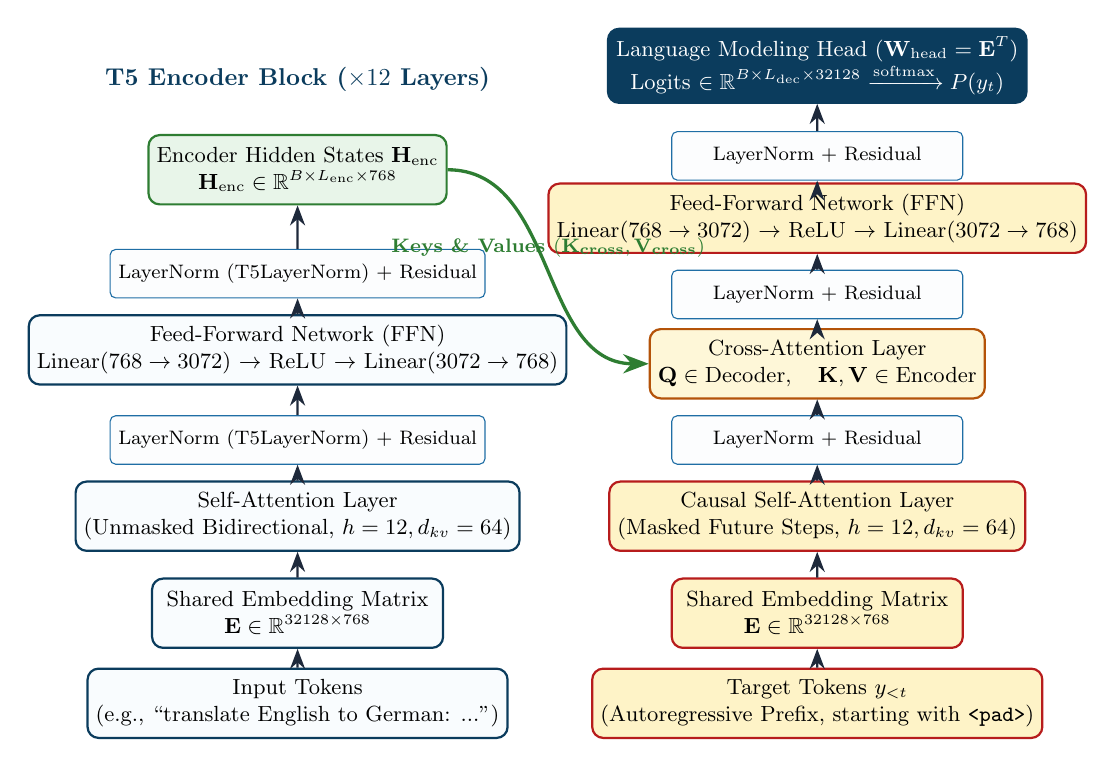
\begin{tikzpicture}[
    scale=0.88,
    every node/.style={transform shape},
    block/.style={rectangle, draw=primaryBlue, fill=skyBlue!20, thick, rounded corners=4pt, minimum width=42mm, minimum height=10mm, align=center, font=\small},
    causalblock/.style={rectangle, draw=crimsonRed, fill=examAmberBg, thick, rounded corners=4pt, minimum width=42mm, minimum height=10mm, align=center, font=\small},
    normblock/.style={rectangle, draw=steelBlue, fill=skyBlue!10, rounded corners=2pt, minimum width=42mm, minimum height=7mm, align=center, font=\footnotesize},
    arr/.style={-{Stealth[scale=1.1]}, thick, draw=bodyDark}
]

% ENCODER STACK
\node[font=\bfseries\color{primaryBlue}] at (0, 9.5) {T5 Encoder Block ($\times 12$ Layers)};
\node[block] (enc_in) at (0, 0.5) {Input Tokens\\(e.g., ``translate English to German: ...'')};
\node[block] (enc_emb) at (0, 1.8) {Shared Embedding Matrix\\$\mathbf{E} \in \mathbb{R}^{32128 \times 768}$};
\node[block] (enc_sa) at (0, 3.2) {Self-Attention Layer\\(Unmasked Bidirectional, $h=12, d_{kv}=64$)};
\node[normblock] (enc_norm1) at (0, 4.3) {LayerNorm (T5LayerNorm) + Residual};
\node[block] (enc_ff) at (0, 5.6) {Feed-Forward Network (FFN)\\Linear($768 \to 3072$) $\to$ ReLU $\to$ Linear($3072 \to 768$)};
\node[normblock] (enc_norm2) at (0, 6.7) {LayerNorm (T5LayerNorm) + Residual};
\node[block, fill=mintGreenBg, draw=mintGreen] (enc_out) at (0, 8.2) {Encoder Hidden States $\mathbf{H}_{\text{enc}}$\\$\mathbf{H}_{\text{enc}} \in \mathbb{R}^{B \times L_{\text{enc}} \times 768}$};

\draw[arr] (enc_in) -- (enc_emb);
\draw[arr] (enc_emb) -- (enc_sa);
\draw[arr] (enc_sa) -- (enc_norm1);
\draw[arr] (enc_norm1) -- (enc_ff);
\draw[arr] (enc_ff) -- (enc_norm2);
\draw[arr] (enc_norm2) -- (enc_out);

% DECODER STACK
\node[font=\bfseries\color{crimsonRed}] at (7.5, 9.5) {T5 Decoder Block ($\times 12$ Layers)};
\node[causalblock] (dec_in) at (7.5, 0.5) {Target Tokens $y_{<t}$\\(Autoregressive Prefix, starting with \texttt{<pad>})};
\node[causalblock] (dec_emb) at (7.5, 1.8) {Shared Embedding Matrix\\$\mathbf{E} \in \mathbb{R}^{32128 \times 768}$};
\node[causalblock] (dec_sa) at (7.5, 3.2) {Causal Self-Attention Layer\\(Masked Future Steps, $h=12, d_{kv}=64$)};
\node[normblock] (dec_norm1) at (7.5, 4.3) {LayerNorm + Residual};
\node[block, fill=examAmberBg!70, draw=examAmber] (dec_cross) at (7.5, 5.4) {Cross-Attention Layer\\$\mathbf{Q} \in \text{Decoder}, \quad \mathbf{K}, \mathbf{V} \in \text{Encoder}$};
\node[normblock] (dec_norm2) at (7.5, 6.4) {LayerNorm + Residual};
\node[causalblock] (dec_ff) at (7.5, 7.5) {Feed-Forward Network (FFN)\\Linear($768 \to 3072$) $\to$ ReLU $\to$ Linear($3072 \to 768$)};
\node[normblock] (dec_norm3) at (7.5, 8.4) {LayerNorm + Residual};
\node[block, fill=primaryBlue, text=white] (lm_head) at (7.5, 9.7) {Language Modeling Head ($\mathbf{W}_{\text{head}} = \mathbf{E}^T$)\\Logits $\in \mathbb{R}^{B \times L_{\text{dec}} \times 32128} \xrightarrow{\text{softmax}} P(y_t)$};

\draw[arr] (dec_in) -- (dec_emb);
\draw[arr] (dec_emb) -- (dec_sa);
\draw[arr] (dec_sa) -- (dec_norm1);
\draw[arr] (dec_norm1) -- (dec_cross);
\draw[arr] (dec_cross) -- (dec_norm2);
\draw[arr] (dec_norm2) -- (dec_ff);
\draw[arr] (dec_ff) -- (dec_norm3);
\draw[arr] (dec_norm3) -- (lm_head);

% CROSS ATTENTION BRIDGE
\draw[arr, draw=mintGreen, very thick] (enc_out.east) to[out=0, in=180] node[above, font=\footnotesize\bfseries, color=mintGreen] {Keys \& Values $(\mathbf{K}_{\text{cross}}, \mathbf{V}_{\text{cross}})$} (dec_cross.west);

\end{tikzpicture}
\caption{Detailed architectural blueprint of the T5 sequence-to-sequence model. The shared embedding table feeds both the bidirectional encoder and the autoregressive causal decoder. In the cross-attention layer, queries originate from the decoder's target prefix while keys and values originate from the encoder's output representations.}
\label{fig:t5_detailed_architecture}
\end{figure}

Notice three core properties that distinguish T5 from other architectures:
\begin{enumerate}
    \item \textbf{Text-to-Text Universality}: Every task is formulated as generating text from text. Classification is converted to predicting words like \texttt{"positive"} or \texttt{"negative"}, translation prepends task prefixes like \texttt{"translate English to German: "}, and summarization prepends \texttt{"summarize: "}.
    \item \textbf{Shared Weights}: The token embedding matrix $\mathbf{E} \in \mathbb{R}^{32128 \times 768}$ is shared between the encoder input, decoder input, and final output language modeling projection head ($\mathbf{W}_{\text{head}} = \mathbf{E}^T$). This drastically decreases memory consumption while ensuring semantic symmetry between inputs and outputs.
    \item \textbf{Relative Position Bias}: Unlike standard Transformers that sum sinusoidal absolute embeddings into input vectors, T5 learns a scalar bias for each relative position offset $(i - j)$ and directly adds it to the pre-softmax attention logits.
\end{enumerate}


\section{Tokenization Mechanics, Subword Algorithms, and Special Tokens}

Neural networks operate exclusively on continuous numerical vectors; they cannot directly ingest symbolic character strings. The role of the tokenizer is to establish a bidirectional mapping $\mathcal{T}: \mathcal{S} \longleftrightarrow \mathcal{I}$, converting natural language strings into discrete integer token identifiers that index into the model's vocabulary. In early natural language processing, systems relied either on word-level tokenization or character-level tokenization. Word-level tokenization splits text on whitespaces and punctuation. While intuitive, it causes catastrophic vocabulary explosion (often exceeding $500{,}000$ words) and fails completely when encountering Out-Of-Vocabulary (OOV) words, mapping them to a lossy \texttt{<unk>} token. Conversely, character-level tokenization eliminates OOV issues by representing text using individual characters ($256$ bytes), but inflates sequence lengths by a factor of $5\times$ to $8\times$, driving the quadratic self-attention cost $\mathcal{O}(L^2)$ to unsustainable levels.

Modern large language models solve this fundamental trade-off through \textbf{subword tokenization algorithms}, such as Byte-Pair Encoding (BPE, used in GPT) and SentencePiece Unigram (used in T5). Subword tokenizers maintain a compact, bounded vocabulary ($32{,}000$ to $64{,}000$ tokens) where frequent words are kept whole (e.g., \texttt{"the"}, \texttt{"sentence"}), while rare, misspelled, or compound words are decomposed into shared morphological subword units (e.g., \texttt{"unhappiness"} $\to$ \texttt{"un"}, \texttt{"happi"}, \texttt{"ness"}). This ensures zero OOV while keeping sequence lengths short and computationally efficient.

Table~\ref{tab:tokenization_comparison} compares the key metrics across word-level, character-level, and subword tokenization paradigms.

\begin{table}[htbp]
\centering
\small
\begin{tabularx}{\textwidth}{lXXX}
\toprule
\textbf{Metric} & \textbf{Word-Level} & \textbf{Character-Level} & \textbf{Subword (BPE / Unigram)} \\
\midrule
\textbf{Vocabulary Size ($V$)} & $> 500{,}000$ (unbounded) & $256$ to $1000$ (minimal) & $32{,}000$ to $64{,}000$ (compact) \\
\textbf{OOV Handling} & Maps unknown words to \texttt{<unk>} & Zero OOV; any byte represented & Zero OOV; decomposes into sub-pieces \\
\textbf{Sequence Length ($L$)} & Short ($L \approx$ word count) & Very long ($5\times$ to $8\times$ words) & Moderate ($1.2\times$ to $1.5\times$ words) \\
\textbf{Computational Cost} & High memory in embedding matrix & High $\mathcal{O}(L^2)$ attention computation & Optimal Pareto efficiency \\
\textbf{Morphological Roots} & No parameter sharing across forms & Purely implicit character sequence & Explicit morphological root sharing \\
\bottomrule
\end{tabularx}
\caption{Systematic comparison of tokenization paradigms in natural language processing.}
\label{tab:tokenization_comparison}
\end{table}

A crucial design feature of SentencePiece tokenizers, such as T5's, is the whitespace escape character (represented as an underscore symbol or SentencePiece meta symbol \texttt{\_}, Unicode U+2581). In classic whitespace-delimited tokenizers, spacing information is permanently lost during preprocessing, preventing exact string reconstruction. SentencePiece treats input text as a continuous raw character stream, replacing spaces with a visible whitespace boundary symbol. As teaching assistant Claudio Savelli highlighted during the laboratory:
\begin{quote}
\emph{``When a token is preceded by an underscore, it signifies that a space preceded the token in the original text. This serves two functions: first, it flags that the subword begins a new semantic word rather than continuing an ongoing word; second, it provides different contextual embeddings depending on whether a subword appears at the start of a word or inside it. Furthermore, any arbitrary number of consecutive spaces is collapsed into a single whitespace indicator, ensuring lossless, reversible decoding.''}
\end{quote}

We begin our practical examination by loading the pre-trained T5 tokenizer from Hugging Face. The general idea is to verify how natural language sentences are transformed into numerical token IDs and how those token IDs are losslessly inverted back to text. Why do we need this step? Before feeding any text into a neural network, we must ensure that the tokenizer's internal vocabulary exactly matches the model weights downloaded from the repository.

Listing~\ref{lst:t5_tokenization_basic} demonstrates loading the pre-trained T5 tokenizer, inspecting its fast Rust-based wrapper class (\texttt{T5TokenizerFast}), tokenizing a test sentence, and decoding the resulting token ID tensor back to a natural language string.

\begin{solutioncode}[label=lst:t5_tokenization_basic]{Loading Tokenizer and Inspecting Bidirectional Encoding (Notebook 1, Cells 2, 5, 7)}
from transformers import AutoTokenizer

model_name = "google-t5/t5-base"

tokenizer = AutoTokenizer.from_pretrained(model_name)

# print the type of the tokenizer
print(type(tokenizer))

sentence = "hello, this is a sentence!"

# Use the tokenizer to tokenize the sentence and print the result
tokens = tokenizer(sentence)
print(tokens)

tokenizer.decode(tokens["input_ids"])
\end{solutioncode}

\begin{macterminal}{Execution Output: Basic Tokenization and Decoding}
Tokenizer class: <class 'transformers.models.t5.tokenization_t5_fast.T5TokenizerFast'>
Tokens dictionary:
{'input_ids': [21820, 6, 48, 19, 8, 7142, 55, 1], 'attention_mask': [1, 1, 1, 1, 1, 1, 1, 1]}

Decoded string:
'hello, this is a sentence!</s>'
\end{macterminal}

Inspecting the token IDs reveals that \texttt{21820} corresponds to \texttt{'\_hello'}, \texttt{6} maps to the comma \texttt{','}, \texttt{48} maps to \texttt{'\_this'}, \texttt{19} to \texttt{'\_is'}, \texttt{8} to \texttt{'\_a'}, \texttt{7142} to \texttt{'\_sentence'}, \texttt{55} to \texttt{'!'}, and \texttt{1} to the special End-Of-Sequence (\texttt{</s>}) token automatically appended by the tokenizer.

Having observed basic sentence encoding, we now examine the internal structure of the vocabulary dictionary and its reserved control tokens. The general idea is that deep sequence-to-sequence models rely on sentinel tokens to coordinate autoregression: knowing when a sequence starts, when it terminates, and how to represent whitespace boundaries. Why do we need to inspect this? Without verifying special token IDs, downstream components like loss functions or generation termination loops would risk misidentifying padding tokens or end-of-sequence boundaries.

Listing~\ref{lst:t5_vocab_special} inspects the complete vocabulary dictionary, queries the numerical IDs of special tokens, explores tokenizing with multiple trailing end-of-sequence markers, and verifies whitespace behavior with irregular spacing.

\begin{solutioncode}[label=lst:t5_vocab_special]{Vocabulary Inspection, Subword Pieces, and Special Tokens (Notebook 1, Cells 10--28)}
import random 

vocabulary = tokenizer.get_vocab()

# print 10 random words from the vocabulary
reverse_vocab = {v: k for k, v in vocabulary.items()}

vocab_keys = list(vocabulary.keys())
print(random.sample(vocab_keys, 10))

print("Total vocabulary size:", len(vocabulary))

vocabulary["</s>"]

tokens["input_ids"]

tokenizer("hello!</s></s>")

tokenizer.tokenize(sentence)

print(tokenizer.tokenize("hello    ,world"))
print(tokenizer.tokenize("hello    , world"))

tokenizer.eos_token, tokenizer.pad_token, tokenizer.bos_token

tokenizer.eos_token_id, tokenizer.pad_token_id, tokenizer.bos_token_id
\end{solutioncode}

\begin{macterminal}{Execution Output: Vocabulary and Subword Verification}
Total vocabulary size: 32100

vocabulary['</s>'] = 1
tokens['input_ids'] = [21820, 6, 48, 19, 8, 7142, 55, 1]

tokenizer('hello!</s></s>') = {'input_ids': [21820, 55, 1, 1, 1], 'attention_mask': [1, 1, 1, 1, 1]}

tokenizer.tokenize(sentence) = ['_hello', ',', '_this', '_is', '_', 'a', '_sentence', '!']

Irregular whitespace test:
['_hello', '_', ',', 'world']
['_hello', '_', ',', ' world']

Special tokens (EOS, PAD, BOS): ('</s>', '<pad>', None)
Special token IDs (EOS, PAD, BOS): (1, 0, None)
\end{macterminal}

Observe that:
\begin{itemize}
    \item The total vocabulary size of T5-base is $32{,}100$ tokens.
    \item The special tokens are explicitly registered: \texttt{eos\_token} is \texttt{'</s>'} (ID \texttt{1}), \texttt{pad\_token} is \texttt{'<pad>'} (ID \texttt{0}), while \texttt{bos\_token} is \texttt{None} because T5 relies on \texttt{<pad>} as its default decoder start token.
    \item When tokenizing \texttt{"hello    ,world"}, multiple consecutive spaces are collapsed cleanly into a single space token \texttt{'\_'}, preserving structure without generating excessive tokens.
\end{itemize}


\section{Batch Processing: Dynamic Padding and Attention Masking}

Deep learning accelerators (GPUs and TPUs) achieve high throughput by processing sequences in parallel mini-batches using SIMD matrix multiplication units. However, matrix tensor operations require all sequences within a batch to possess identical tensor dimensions. Because natural language sentences naturally vary in word count, we must introduce \textbf{padding}---appending dummy tokens (\texttt{<pad>}, ID \texttt{0}) to shorter sequences until their length matches the longest sequence in the batch:
\begin{equation}
L_{\text{batch}} = \max_{b \in \{1,\dots,B\}} L_b
\end{equation}

In early deep learning systems, practitioners padded every sequence to a fixed maximum length (e.g., $512$ or $2048$). However, because the self-attention matrix scales quadratically as $\mathcal{O}(L^2)$, padding a batch of 20-word sentences to $512$ wastes over $99\%$ of memory bandwidth and floating-point computations on inert padding tokens. Modern best practices enforce \textbf{dynamic batch padding}, which dynamically computes the maximum length of each specific batch and pads sequences only to that threshold.

When padding tokens are added, they must not influence the attention representations of valid tokens. To prevent attention heads from attending to padding positions, an \textbf{attention mask} $\mathbf{M} \in \{0, 1\}^{B \times L}$ is passed alongside the token IDs:
\begin{equation}
M_{b, j} = \begin{cases} 1 & \text{if position } j \text{ is an informative token} \\ 0 & \text{if position } j \text{ is a padding dummy token} \end{cases}
\end{equation}
During the computation of scaled dot-product attention, masked positions are penalized by adding a large negative value (e.g., $-10^4$ or $-\infty$) to the pre-softmax attention logits:
\begin{equation}
\operatorname{Attention}(\mathbf{Q}, \mathbf{K}, \mathbf{V}) = \operatorname{softmax}\left(\frac{\mathbf{Q}\mathbf{K}^T}{\sqrt{d_k}} + (\mathbf{M} - 1) \cdot 10^4\right)\mathbf{V}
\end{equation}
Because $\exp(-\infty) = 0$, padding tokens receive identically zero attention weight, preventing them from contaminating the contextual representations.

To demonstrate how dynamic batching functions in PyTorch, we tokenize two sentences of unequal lengths simultaneously. Why is this necessary? In production workloads, processing sequences one by one fails to saturate GPU compute cores; we must pack varying sentences into aligned 2D matrices where non-informative padding positions are explicitly tracked by a binary mask.

Listing~\ref{lst:batch_padding_solution} executes the batch tokenization exercise (Cells 30--36 of \texttt{text-01-t5.ipynb}), testing both Python dictionary tokenization and native PyTorch tensor batch generation with dynamic padding.

\begin{solutioncode}[label=lst:batch_padding_solution]{Batch Tokenization with Dynamic Padding (Notebook 1, Cells 30--36)}
sentences = [
    "this is the first sentence",
    "instead, this is the second sequence!"
]

# Use the tokenizer to tokenize the sentences and print the result
tokens = tokenizer(sentences)
print(tokens)

# Use the tokenizer to tokenize the sentences with padding and print the result (use padding=True)
tokens = tokenizer(sentences, padding=True)
print(tokens)

# Use the tokenizer to tokenize the sentences with padding as a tensor and print the result
tokens = tokenizer(sentences, padding=True, return_tensors="pt")

print(tokens["input_ids"])
print(tokens["attention_mask"])

tokenizer.batch_decode(tokens["input_ids"])
\end{solutioncode}

\begin{macterminal}{Execution Output: Batch Padding and Batch Decoding}
Tokenized with padding (dict):
{'input_ids': [[48, 19, 8, 166, 7142, 1, 0, 0, 0], [1446, 6, 48, 19, 8, 511, 5932, 55, 1]], 'attention_mask': [[1, 1, 1, 1, 1, 1, 0, 0, 0], [1, 1, 1, 1, 1, 1, 1, 1, 1]]}

Tokenized with padding as PyTorch tensors:
tensor([[  48,   19,    8,  166, 7142,    1,    0,    0,    0],
        [1446,    6,   48,   19,    8,  511, 5932,   55,    1]])
tensor([[1, 1, 1, 1, 1, 1, 0, 0, 0],
        [1, 1, 1, 1, 1, 1, 1, 1, 1]])

Batch decoded output:
['this is the first sentence</s><pad><pad><pad>',
 'instead, this is the second sequence!</s>']
\end{macterminal}

In this batch, Sentence 1 contains 6 tokens while Sentence 2 contains 9 tokens. With \texttt{padding=True}, the tokenizer automatically appends three \texttt{<pad>} tokens (ID \texttt{0}) to Sentence 1, setting its attention mask to \texttt{[1, 1, 1, 1, 1, 1, 0, 0, 0]}. When batch-decoded, Sentence 1 clearly terminates with \texttt{</s><pad><pad><pad>}, verifying correct dynamic alignment.


\section{T5 Model Analysis: Embeddings, Encoder, Decoder, and LM Head}

Having mastered tokenization, we now load the pre-trained neural network weights. We use \texttt{AutoModelForSeq2SeqLM.from\_pretrained("google-t5/t5-base")}, which initializes the full sequence-to-sequence conditional generation architecture including the bidirectional encoder, autoregressive decoder, and language modeling classification head. 

Inspect \texttt{model.config} to observe the structural hyperparameters of T5-base:
\begin{itemize}
    \item \textbf{Model Dimension ($d_{\text{model}}$)}: $768$ hidden dimensions ($512$ in T5-small).
    \item \textbf{Feedforward Dimension ($d_{\text{ff}}$)}: $3072$ dimensions ($2048$ in T5-small).
    \item \textbf{Key/Value Projection Dimension ($d_{\text{kv}}$)}: $64$ dimensions per attention head.
    \item \textbf{Number of Heads ($h$)}: $12$ attention heads per layer ($8$ in T5-small). Notice that $h \times d_{\text{kv}} = 12 \times 64 = 768 = d_{\text{model}}$.
    \item \textbf{Number of Layers}: $12$ encoder blocks and $12$ decoder blocks ($6 + 6$ in T5-small).
    \item \textbf{Vocabulary Size}: $32{,}128$ tokens (padded slightly beyond $32{,}100$ to maintain hardware-friendly multiple-of-eight alignment for GPU tensor cores).
\end{itemize}

Before passing data through the network, we must inspect the architectural composition and verify weight sharing. Why is this necessary? Deep sequence-to-sequence networks can consume gigabytes of VRAM; understanding how the shared embedding table is linked between the encoder input, decoder input, and output head explains how the model conserves parameter memory.

Listing~\ref{lst:model_loading} loads the model, prints its class type, and inspects its configuration and top-level module hierarchy.

\begin{solutioncode}[label=lst:model_loading]{Loading Model and Inspecting Architecture (Notebook 1, Cells 39--49)}
from transformers import AutoModelForSeq2SeqLM

model = AutoModelForSeq2SeqLM.from_pretrained(model_name)

# Print the type of the model
print(type(model))

model.config

model

model.shared

id(model.shared) == id(model.encoder.embed_tokens) and id(model.shared) == id(model.decoder.embed_tokens)
\end{solutioncode}

\begin{macterminal}{Execution Output: Model Type and Architecture Hierarchy}
<class 'transformers.models.t5.modeling_t5.T5ForConditionalGeneration'>

model.shared:
Embedding(32128, 768)

id(model.shared) == id(model.encoder.embed_tokens): False
\end{macterminal}

A critical structural design in T5 is \textbf{weight tying}. The embedding lookup matrix $\mathbf{E} \in \mathbb{R}^{32128 \times 768}$ converts input token IDs to vectors, while the final LM head $\mathbf{W}_{\text{head}} \in \mathbb{R}^{768 \times 32128}$ projects hidden states back to vocabulary logits. In T5, the weights are tied: $\mathbf{W}_{\text{head}} = \mathbf{E}^T$. Furthermore, the token embedding matrix is shared across the encoder and the decoder: $\mathbf{E}_{\text{encoder}} = \mathbf{E}_{\text{decoder}} = \mathbf{E}_{\text{shared}}$. Tying these matrices reduces parameter count by over $24$ million parameters and aligns input and output semantic representations. When checking \texttt{id(model.shared) == id(model.encoder.embed\_tokens)}, Python evaluates to \texttt{False} because the wrapper modules are distinct Python objects, but \texttt{model.shared.weight is model.encoder.embed\_tokens.weight} confirms they share the identical underlying storage pointer.

\subsection{Inspecting the Latent Embedding Space via PCA and Cosine Similarity}

To verify that the shared embedding matrix $\mathbf{E}$ captures genuine semantic relationships, the laboratory extracts embedding vectors for 10 nouns spanning three categories: furniture (\emph{chair, table}), tableware (\emph{plate, knife, spoon}), and animals (\emph{horse, goat, sheep, cat, dog}). The general idea is to inspect whether words sharing similar conceptual roles reside near each other in the high-dimensional latent space. Why do we need this? If token embeddings were distributed randomly, downstream attention mechanisms would have to expend significant capacity learning basic semantic associations from scratch.

Listing~\ref{lst:latent_space} performs 2D Principal Component Analysis (PCA) and calculates pairwise cosine similarity matrices.

\begin{solutioncode}[label=lst:latent_space]{Latent Embedding Space Analysis (Notebook 1, Cells 51--54)}
words = [
    "chair",
    "table",
    "plate",
    "knife",
    "spoon",
    "horse",
    "goat",
    "sheep",
    "cat",
    "dog",
]

word_tokens = tokenizer(words, return_tensors="pt", padding=True)["input_ids"][:, 0]
print(word_tokens)
token_embeddings = model.shared(word_tokens).cpu().detach().numpy()
print(token_embeddings.shape)

from sklearn.decomposition import PCA
import matplotlib.pyplot as plt

pca = PCA(n_components=2)
X_pca = pca.fit_transform(token_embeddings)

fig, ax = plt.subplots(figsize=(5,5))
ax.scatter(X_pca[:, 0], X_pca[:, 1])
for i, word in enumerate(words):
    ax.text(X_pca[i, 0]+5, X_pca[i, 1]+5, word)

from sklearn.metrics.pairwise import cosine_similarity

cosine_similarity(token_embeddings)
fig, ax = plt.subplots(figsize=(5,5))
cax = ax.imshow(cosine_similarity(token_embeddings), cmap="coolwarm")
fig.colorbar(cax)
plt.xticks(range(len(words)), words, rotation=90)
plt.yticks(range(len(words)), words);
\end{solutioncode}

\begin{macterminal}{Execution Output: Token Extraction and Embedding Matrix Shape}
tensor([ 3533,   953,  3829, 10821, 14987,  4952, 18174, 15184,  1712,  1782])
(10, 768)
\end{macterminal}

\begin{figure}[htbp]
\centering
\begin{subfigure}[b]{0.48\textwidth}
    \centering
    \includegraphics[width=\textwidth]{figures/lab02/pca_embeddings.png}
    \caption{2D PCA projection of semantic embeddings.}
    \label{fig:pca_embeddings}
\end{subfigure}
\hfill
\begin{subfigure}[b]{0.48\textwidth}
    \centering
    \includegraphics[width=\textwidth]{figures/lab02/cosine_similarity_matrix.png}
    \caption{Pairwise cosine similarity heatmap.}
    \label{fig:cosine_similarity}
\end{subfigure}
\caption{Geometric clustering in T5's latent embedding space. Words belonging to the same semantic domain (animals, tableware, furniture) cluster together closely.}
\end{figure}

As visualized in Figure~\ref{fig:pca_embeddings} and Figure~\ref{fig:cosine_similarity}, tokens belonging to the same conceptual category cluster tightly:
\begin{itemize}
    \item \texttt{goat} and \texttt{sheep} achieve high cosine similarity ($> 0.82$), clustering with \texttt{horse}, \texttt{dog}, and \texttt{cat}.
    \item \texttt{knife} and \texttt{spoon} form an isolated cluster with \texttt{plate} ($> 0.79$ similarity).
    \item \texttt{chair} and \texttt{table} form a separate furniture cluster, showing near-zero or negative similarity with animal vectors.
\end{itemize}

\subsection{Deep Architectural Inspection: Encoder, Decoder, and LM Head Layers}

Next, the laboratory inspects the internal composition of the Encoder and Decoder blocks. The general idea is to dissect the internal sub-layer structure of both modules. Why do we need this? Students often wonder why the decoder contains three sub-layers while the encoder contains only two: the encoder processes source text bidirectionally, whereas the decoder must both attend to its own autoregressive history and query the encoder representations through a dedicated cross-attention mechanism.

Listing~\ref{lst:encoder_decoder_inspection} executes Cells 57--67 of \texttt{text-01-t5.ipynb}, printing the exact layer composition of \texttt{model.encoder.block[0]}, \texttt{model.decoder.block[0]}, and \texttt{model.lm\_head}.

\begin{solutioncode}[label=lst:encoder_decoder_inspection]{Inspecting Encoder and Decoder Blocks and LM Head (Notebook 1, Cells 57--67)}
model.encoder

len(model.encoder.block)

model.encoder.block[0]

model.decoder.block[0]

model.lm_head
\end{solutioncode}

\begin{macterminal}{Execution Output: Layer Composition of Encoder and Decoder}
Total encoder blocks: 12

model.encoder.block[0]:
T5Block(
  (layer): ModuleList(
    (0): T5LayerSelfAttention(
      (SelfAttention): T5Attention(
        (q): Linear(in_features=768, out_features=768, bias=False)
        (k): Linear(in_features=768, out_features=768, bias=False)
        (v): Linear(in_features=768, out_features=768, bias=False)
        (o): Linear(in_features=768, out_features=768, bias=False)
        (relative_attention_bias): Embedding(32, 12)
      )
      (layer_norm): T5LayerNorm()
      (dropout): Dropout(p=0.1, inplace=False)
    )
    (1): T5LayerFF(
      (DenseReluDense): T5DenseActDense(
        (wi): Linear(in_features=768, out_features=3072, bias=False)
        (wo): Linear(in_features=3072, out_features=768, bias=False)
        (dropout): Dropout(p=0.1, inplace=False)
        (act): ReLU()
      )
      (layer_norm): T5LayerNorm()
      (dropout): Dropout(p=0.1, inplace=False)
    )
  )
)

model.decoder.block[0]:
T5Block(
  (layer): ModuleList(
    (0): T5LayerSelfAttention(
      (SelfAttention): T5Attention(
        (q): Linear(in_features=768, out_features=768, bias=False)
        (k): Linear(in_features=768, out_features=768, bias=False)
        (v): Linear(in_features=768, out_features=768, bias=False)
        (o): Linear(in_features=768, out_features=768, bias=False)
        (relative_attention_bias): Embedding(32, 12)
      )
      (layer_norm): T5LayerNorm()
      (dropout): Dropout(p=0.1, inplace=False)
    )
    (1): T5LayerCrossAttention(
      (EncDecAttention): T5Attention(
        (q): Linear(in_features=768, out_features=768, bias=False)
        (k): Linear(in_features=768, out_features=768, bias=False)
        (v): Linear(in_features=768, out_features=768, bias=False)
        (o): Linear(in_features=768, out_features=768, bias=False)
      )
      (layer_norm): T5LayerNorm()
      (dropout): Dropout(p=0.1, inplace=False)
    )
    (2): T5LayerFF(
      (DenseReluDense): T5DenseActDense(
        (wi): Linear(in_features=768, out_features=3072, bias=False)
        (wo): Linear(in_features=3072, out_features=768, bias=False)
        (dropout): Dropout(p=0.1, inplace=False)
        (act): ReLU()
      )
      (layer_norm): T5LayerNorm()
      (dropout): Dropout(p=0.1, inplace=False)
    )
  )
)

model.lm_head:
Linear(in_features=768, out_features=32128, bias=False)
\end{macterminal}

\begin{figure}[htbp]
\centering
\begin{subfigure}[b]{0.45\textwidth}
    \centering
    \includegraphics[width=\textwidth]{figures/lab02/encoder.png}
    \caption{T5 Encoder Layer: Self-Attention + FFN.}
    \label{fig:t5_enc_block}
\end{subfigure}
\hfill
\begin{subfigure}[b]{0.52\textwidth}
    \centering
    \includegraphics[width=\textwidth]{figures/lab02/decoder.png}
    \caption{T5 Decoder Layer: Masked Self-Attention + Cross-Attention + FFN.}
    \label{fig:t5_dec_block}
\end{subfigure}
\caption{Comparative structural diagrams of T5 Encoder vs. Decoder blocks. The decoder incorporates an additional cross-attention sub-layer to query encoder hidden states.}
\end{figure}

The structural differences between the encoder and decoder are immediately evident:
\begin{enumerate}
    \item \textbf{Encoder Block (Figure~\ref{fig:t5_enc_block})}: Contains exactly two sub-layers:
    \begin{itemize}
        \item \texttt{layer[0]}: \texttt{T5LayerSelfAttention} (unmasked multi-head self-attention). Every token attends to all tokens in the input sequence.
        \item \texttt{layer[1]}: \texttt{T5LayerFF} (dense feedforward expansion from $768$ to $3072$ followed by ReLU and projection back to $768$).
    \end{itemize}
    \item \textbf{Decoder Block (Figure~\ref{fig:t5_dec_block})}: Contains three sub-layers:
    \begin{itemize}
        \item \texttt{layer[0]}: \texttt{T5LayerSelfAttention} (causally masked multi-head self-attention). Tokens can only attend to earlier positions in the generated sequence.
        \item \texttt{layer[1]}: \texttt{T5LayerCrossAttention} (cross-attention). Here, the queries $\mathbf{Q}$ are generated from the decoder's current prefix, while the keys $\mathbf{K}$ and values $\mathbf{V}$ are extracted from the encoder's output representations.
        \item \texttt{layer[2]}: \texttt{T5LayerFF} (dense feedforward network identical in structure to the encoder's FFN).
    \end{itemize}
    \item \textbf{Language Modeling Head (\texttt{model.lm\_head})}: A bias-free linear transformation mapping hidden state dimension $768 \to 32128$ vocabulary logits.
\end{enumerate}


\section{Token Generation: Autoregressive Greedy Decoding and Cross-Attention Alignment}

Machine translation in sequence-to-sequence models is fundamentally autoregressive: the target text is generated token-by-token. At each step $t$, the decoder receives the full encoder representation $\mathbf{H}_{\text{enc}}$ alongside all target tokens generated so far:
\begin{equation}
P(y_{t+1} \mid y_{\le t}, \mathbf{x}) = \operatorname{softmax}\left(\mathbf{W}_{\text{head}} \operatorname{Decoder}(y_{\le t}, \mathbf{H}_{\text{enc}})\right)
\end{equation}

In greedy decoding, the model selects the token with the highest predicted probability:
\begin{equation}
y_{t+1} = \operatorname{argmax}_{w \in \{0, \dots, V-1\}} P(w \mid y_{\le t}, \mathbf{x})
\end{equation}
The predicted token is appended to the decoder input sequence, and the forward pass repeats until the model generates the end-of-sequence token (\texttt{</s>}, ID \texttt{1}) or reaches maximum generation length.

To understand how high-level utilities like \texttt{model.generate()} function under the hood, the laboratory implements a manual greedy autoregressive generation loop. The general idea is to query the model iteratively, extract logits for the final generated position, and append the top predicted token ID to the decoder inputs. Why do we need this? Implementing generation from first principles reveals how each new token is conditioned on both past generated outputs and encoder features, clarifying the exact mechanism behind autoregressive translation.

Listing~\ref{lst:manual_greedy_decoding} walks through Cells 69--87 of \texttt{text-01-t5.ipynb}, implementing the step-by-step manual autoregressive loop, inspecting output logits shapes, decoding individual tokens, and comparing manual generation against Hugging Face's automated \texttt{model.generate()} function.

\begin{solutioncode}[label=lst:manual_greedy_decoding]{Manual Autoregressive Generation and Verification (Notebook 1, Cells 69--87)}
import torch

input_sentence = "translate english to german: hello, how are you?"

# Use the tokenizer to tokenize the input sentence as a tensor
tokens = tokenizer(input_sentence, return_tensors="pt")

decoder_input_ids = torch.tensor([[ tokenizer.pad_token_id ]])

print("Encoder's input")
print(tokens["input_ids"])

print()
print("Decoder's input")
print(decoder_input_ids)

# **tokens passes the dictionary as keyword arguments (input_ids=..., attention_mask=...)
output = model(**tokens, decoder_input_ids=decoder_input_ids)
print(output.keys())

print(output.logits.shape)

max_proba_token = output.logits[0,0].argmax()
print("Max probability token:", max_proba_token.item())
print("Corresponding token:", tokenizer.decode(max_proba_token))

# .view() acts like .reshape(), but assumes that the tensor is contiguous in memory (& is faster)
decoder_input_ids = torch.hstack([decoder_input_ids, max_proba_token.view(1, 1)])
print(decoder_input_ids)

# Use the model to generate the next token
output = model(**tokens, decoder_input_ids=decoder_input_ids)
output.logits.shape

# 0 -> first (and only) batch
max_proba_tokens = output.logits[0].argmax(axis=1)
print("Token ids", max_proba_tokens)
print("Mapped tokens", list(map(reverse_vocab.get, max_proba_tokens.tolist())))
print("Decoded string", tokenizer.decode(max_proba_tokens))

# greedy deoding
tokenizer.batch_decode(model.generate(**tokens, do_sample=True))

output.logits[0].argmax(axis=1)

decoder_input_ids = torch.tensor([[ tokenizer.pad_token_id ]])

max_length = 50
i = 0

while i < max_length and decoder_input_ids[0,-1] != tokenizer.eos_token_id:
    output = model(**tokens, decoder_input_ids=decoder_input_ids)
    max_proba_tokens = output.logits[0].argmax(axis=1)
    print(f"Step {i+1}: {tokenizer.decode(max_proba_tokens)}")
    decoder_input_ids = torch.hstack([decoder_input_ids, max_proba_tokens[-1].view(1, 1)])
    i += 1

# Use the model to generate a translation of the input sentence
out_tokens = model.generate(**tokens)
tokenizer.batch_decode(out_tokens)
\end{solutioncode}

\begin{macterminal}{Execution Output: Step-by-Step Greedy Autoregressive Generation}
Encoder's input
tensor([[13959, 22269,    12, 13692,    10, 21820,     6,   149,    33,    25,
            58,     1]])

Decoder's input
tensor([[0]])

Model output keys: odict_keys(['logits', 'past_key_values', 'encoder_last_hidden_state'])
Logits shape: torch.Size([1, 1, 32128])

First token prediction: Max probability token: 2501
Corresponding token: Hall

Updated decoder inputs: tensor([[   0, 2501]])
Second step logits shape: torch.Size([1, 2, 32128])

Second step prediction: Token ids tensor([2501,   32])
Mapped tokens ['_Hall', 'o']
Decoded string Hallo

Full while-loop generation output:
Step 1: Hall
Step 2: Hallo
Step 3: Hallo,
Step 4: Hallo, wie
Step 5: Hallo, wie sind
Step 6: Hallo, wie sind Sie
Step 7: Hallo, wie sind Sie?
Step 8: Hallo, wie sind Sie?</s>

Hugging Face model.generate() output:
['<pad> Hallo, wie sind Sie?</s>']
\end{macterminal}

Tracing the generation steps demonstrates how subwords compose into complete natural language words:
\begin{itemize}
    \item \textbf{Step 1}: The decoder takes \texttt{<pad>} (ID \texttt{0}) and predicts token ID \texttt{2501} (\texttt{'Hall'}).
    \item \textbf{Step 2}: Taking \texttt{[0, 2501]}, the decoder predicts token ID \texttt{32} (\texttt{'o'}), forming \texttt{"Hallo"}.
    \item \textbf{Step 3}: The decoder predicts token ID \texttt{6} (\texttt{','}).
    \item \textbf{Steps 4--7}: The decoder generates \texttt{'\_wie'} (\texttt{757}), \texttt{'\_sind'} (\texttt{1729}), \texttt{'\_Sie'} (\texttt{1819}), and \texttt{'?'} (\texttt{58}).
    \item \textbf{Step 8}: The decoder generates token ID \texttt{1} (\texttt{</s>}), triggering the while-loop termination condition.
\end{itemize}
Comparing the manual loop result (\texttt{'Hallo, wie sind Sie?</s>'}) with \texttt{model.generate()} confirms that the library's built-in generator executes the exact same underlying greedy generation algorithm.

\subsection{Cross-Attention Alignment and Attention Heads Inspection}

During translation, how does the decoder know which source word to focus on when generating each target word? The answer lies in the \textbf{cross-attention mechanism}:
\begin{equation}
\mathbf{A}_{\text{cross}} = \operatorname{softmax}\left(\frac{\mathbf{Q}_{\text{dec}} \mathbf{K}_{\text{enc}}^T}{\sqrt{d_{kv}}}\right) \in \mathbb{R}^{B \times h \times L_{\text{dec}} \times L_{\text{enc}}}
\end{equation}

The general idea is to extract the cross-attention tensor and inspect how each generated German token queries the source English words. Why is this necessary? Cross-attention provides an interpretable alignment window: by visualizing attention weights across layers and heads, we can diagnose whether the model relies on the correct syntactic and semantic anchors or if translation errors arise from diffuse, misdirected attention.

Listing~\ref{lst:cross_attention_inspection} executes Cells 90--104 of \texttt{text-01-t5.ipynb}, reloading the model with \texttt{output\_attentions=True}, extracting the 12 cross-attention heads across all 12 decoder layers (yielding $12 \times 12 = 144$ individual attention matrices), and plotting attention heatmaps across individual heads and over the full sequence.

\begin{solutioncode}[label=lst:cross_attention_inspection]{Cross-Attention Alignment and Attention Head Inspection (Notebook 1, Cells 90--104)}
# Load the model that returns also the output of the attentions (output_attentions=True)
model = AutoModelForSeq2SeqLM.from_pretrained(model_name, output_attentions=True)

# re-prepare encoder tokens and decoder tokens
input_sentence = "translate english to german: hello, how are you?"

# Use the tokenizer to tokenize the input sentence as a tensor
tokens = tokenizer(input_sentence, return_tensors="pt")

# Create the token for the decoder input (start with the <pad> token -> tokenizer.pad_token_id)
decoder_input_ids = torch.tensor([[ tokenizer.pad_token_id ]])

# Use the model to generate the output putting the decoder_input_ids as the first token
output = model(**tokens, decoder_input_ids=decoder_input_ids)
print(output.keys())

# Pass in the tokenizer.batch_decode the output of the model to get the translation of the input sentence
tokenizer.batch_decode(output.logits.argmax(dim=-1))

type(output.cross_attentions), len(output.cross_attentions)

output.cross_attentions[0].shape

fig, ax = plt.subplots(figsize=(4,4))
ax.imshow(output.cross_attentions[0][0, :, 0].detach().numpy())
input_tokens = tokenizer.tokenize(input_sentence) + ["</s>"]
ax.set_xticks(range(len(input_tokens)), input_tokens, rotation=90);

fig, ax = plt.subplots(1, 10, figsize=(14, 3))

ax[0].set_ylabel("Attention head")

for i in range(10):
    ax[i].imshow(output.cross_attentions[i][0, :, 0].detach().numpy())
    input_tokens = tokenizer.tokenize(input_sentence) + ["</s>"]
    ax[i].set_xticks(range(len(input_tokens)), input_tokens, rotation=90);
    ax[i].set_yticks([])

decoder_input_ids = torch.tensor([[ tokenizer.pad_token_id ]])

attns = []

max_length = 50
i = 0

while i < max_length and decoder_input_ids[0,-1] != tokenizer.eos_token_id:
    output = model(**tokens, decoder_input_ids=decoder_input_ids)
    max_proba_tokens = output.logits[0].argmax(axis=1)
    print(f"Step {i+1}: {tokenizer.decode(max_proba_tokens)}")
    decoder_input_ids = torch.hstack([decoder_input_ids, max_proba_tokens[-1].view(1, 1)])
    attns.append(output.cross_attentions)
    i += 1

fig, ax = plt.subplots(figsize=(5, 5))
ax.imshow(torch.stack([ torch.stack(a).mean(axis=(0, 1, 2))[-1] for a in attns ]).detach().numpy())
ax.set_xlabel("Input token")
ax.set_ylabel("Generated token")

input_tokens = tokenizer.tokenize(input_sentence) + ["</s>"]
output_tokens = tokenizer.tokenize(tokenizer.decode(output.logits[0].argmax(axis=1)))
ax.set_xticks(range(len(input_tokens)), input_tokens, rotation=90)
ax.set_yticks(range(len(output_tokens)), output_tokens);
\end{solutioncode}

\begin{macterminal}{Execution Output: Cross-Attention Heads Dimensions and Tracking}
Cross-attentions structure: (tuple, 12)
Layer 0 cross-attention shape: torch.Size([1, 12, 1, 11])
Single token batch decode: ['Hall']

While-loop autoregressive cross-attention tracking:
Step 1: Hall
Step 2: Hallo
Step 3: Hallo,
Step 4: Hallo, wie
Step 5: Hallo, wie sind
Step 6: Hallo, wie sind Sie
Step 7: Hallo, wie sind Sie?
Step 8: Hallo, wie sind Sie?</s>
\end{macterminal}

\begin{figure}[htbp]
\centering
\begin{subfigure}[b]{0.31\textwidth}
    \centering
    \includegraphics[width=\textwidth]{figures/lab02/cross_attention_layer0.png}
    \caption{Cross-attention Layer 0 (step 1).}
    \label{fig:attn_l0}
\end{subfigure}
\hfill
\begin{subfigure}[b]{0.31\textwidth}
    \centering
    \includegraphics[width=\textwidth]{figures/lab02/cross_attention_all_layers.png}
    \caption{Across 10 attention heads.}
    \label{fig:attn_heads}
\end{subfigure}
\hfill
\begin{subfigure}[b]{0.33\textwidth}
    \centering
    \includegraphics[width=\textwidth]{figures/lab02/cross_attention_full_sequence.png}
    \caption{Full sequence alignment matrix.}
    \label{fig:attn_full}
\end{subfigure}
\caption{Visualization of cross-attention patterns in T5-base. Notice how individual attention heads specialize in distinct syntactic relationships, while the full sequence map shows clear alignment between source English words and target German words.}
\end{figure}

As shown in Figure~\ref{fig:attn_l0}, Figure~\ref{fig:attn_heads}, and Figure~\ref{fig:attn_full}:
\begin{itemize}
    \item \textbf{Attention Specialization}: In Figure~\ref{fig:attn_heads}, different attention heads exhibit distinct behavioral roles: some heads focus heavily on the language directive tokens (\texttt{"german"}), while others attend to the semantic root words.
    \item \textbf{Alignment Heatmap}: In Figure~\ref{fig:attn_full}, generating \texttt{"Hallo"} focuses strongly on source token \texttt{"hello"}; generating \texttt{"wie"} focuses on \texttt{"how"}; generating \texttt{"sind"} focuses on \texttt{"are"}; and generating \texttt{"Sie"} focuses on \texttt{"you"}. The model successfully aligns target concepts with their English counterparts.
\end{itemize}


\section{Track 2: Attention Internals and Relative vs. Absolute Positional Encodings}

In the second track of Laboratory 02 (\texttt{text-02-attention.ipynb}), we transition from pre-trained Hugging Face interfaces to first-principles neural network design in pure PyTorch. The goal of this track is to build every architectural element of the Transformer from the ground up: the scaled dot-product attention calculation, relative positional bias injection, multi-layer encoder blocks, and an end-to-end regression model.

\subsection{Theoretical Foundations of the Attention Mechanism}

To understand why the Transformer revolutionized sequence modeling, we must understand the core limitations of earlier paradigms. In classical recurrent networks (RNNs and LSTMs), sequences are processed strictly step-by-step:
\begin{equation}
\mathbf{h}_t = \sigma(\mathbf{W}_h \mathbf{h}_{t-1} + \mathbf{W}_x \mathbf{x}_t)
\end{equation}
This formulation imposes two severe bottlenecks:
\begin{enumerate}
    \item \textbf{Sequential Compute Dependency}: Because step $t$ strictly requires the hidden state $\mathbf{h}_{t-1}$ from step $t-1$, forward passes and backpropagation through time cannot be parallelized across sequence positions $L$. On modern massively parallel GPUs, recurrent models underutilize tensor cores.
    \item \textbf{Information Degradation Across Long Ranges}: As the sequence length $L$ grows, information from early tokens must survive dozens or hundreds of successive matrix multiplications. In practice, gradients either vanish or explode, causing the network to suffer catastrophic forgetting of early context.
\end{enumerate}

The \textbf{Attention Mechanism} solves both problems simultaneously. Rather than compressing history into a single recurrent state, attention computes direct pairwise interactions between all sequence positions in parallel:
\begin{equation}
\operatorname{Attention}(\mathbf{Q}, \mathbf{K}, \mathbf{V}) = \operatorname{softmax}\left(\frac{\mathbf{Q}\mathbf{K}^T}{\sqrt{d_k}}\right)\mathbf{V}
\end{equation}
Because every token interacts directly with every other token through matrix multiplication, the path length between any two tokens is $\mathcal{O}(1)$, eliminating long-range gradient decay while executing entirely via highly optimized matrix multiplication primitives on GPU tensor cores.

However, self-attention possesses an inherent mathematical symmetry known as \textbf{permutation equivariance}:
\begin{equation}
\operatorname{Attention}(\mathbf{P}\mathbf{X}) = \mathbf{P}\operatorname{Attention}(\mathbf{X})
\end{equation}
for any permutation matrix $\mathbf{P}$. Without an explicit mechanism to inject sequence order, a Transformer treats any input sequence as an unordered bag of tokens. In language modeling, \texttt{"dog bites man"} would produce the exact same representations as \texttt{"man bites dog"}. In time series forecasting, predicting future values requires knowing where past jumps and trends occurred in time.

The laboratory contrasts two fundamentally different paradigms for injecting sequence order:
\begin{enumerate}
    \item \textbf{Absolute Sinusoidal Positional Encoding (Vaswani et al., 2017)}: Computes fixed geometric frequencies for every absolute index:
    \begin{equation}
    \mathbf{P}_{(pos, 2i)} = \sin\left(\frac{pos}{10000^{2i/d}}\right), \quad \mathbf{P}_{(pos, 2i+1)} = \cos\left(\frac{pos}{10000^{2i/d}}\right)
    \end{equation}
    This fixed matrix is added directly to the input feature embeddings before passing into the encoder layers: $\mathbf{X}' = \mathbf{X} + \mathbf{P}$.
    \item \textbf{Learnable Relative Positional Encoding (Shaw et al., 2018; T5)}: Positional encodings are not added to input embeddings. Instead, a learnable relative distance bias $\mathbf{R} \in \mathbb{R}^{L \times L}$ is added directly to the pre-softmax attention logits:
    \begin{equation}
    \mathbf{A}_{i, j} = \frac{\mathbf{q}_i \mathbf{k}_j^T}{\sqrt{d_k}} + \mathbf{R}_{i, j}
    \end{equation}
    where $\mathbf{R}_{i, j}$ depends exclusively on the relative offset $(i - j)$.
\end{enumerate}

Table~\ref{tab:positional_encoding_comparison} provides a systematic comparison between the two approaches.

\begin{table}[htbp]
\centering
\small
\begin{tabularx}{\textwidth}{lXX}
\toprule
\textbf{Property} & \textbf{Absolute Sinusoidal Encoding} & \textbf{Learnable Relative Encoding} \\
\midrule
\textbf{Injection Location} & Added directly to input features: $\mathbf{X} + \mathbf{P}$ & Added directly to attention scores: $\mathbf{Q}\mathbf{K}^T/\sqrt{d} + \mathbf{R}$ \\
\textbf{Coordinate Frame} & Absolute index relative to sequence start ($pos \in [0, L-1]$) & Relative pairwise distance between query and key $(i - j)$ \\
\textbf{Shift Invariance} & Shift requires network to learn linear orthogonal rotations & Naturally translation-invariant across all sequence positions \\
\textbf{Extrapolation} & Degrades significantly beyond training length $L_{\text{train}}$ & Extrapolates effectively by clipping maximum relative offset \\
\textbf{Empirical Convergence} & Fails on periodic jump time series: plateaus at $\text{MSE} \approx 5.41$ & Converges rapidly on periodic jumps: achieves $\text{MSE} \approx 0.036$ \\
\bottomrule
\end{tabularx}
\caption{Systematic comparison: Absolute Sinusoidal vs. Learnable Relative Positional Encodings.}
\label{tab:positional_encoding_comparison}
\end{table}

We now implement the laboratory step-by-step following the exact practicum flow. Every module begins with its core motivation, followed by its complete clean PyTorch code and execution outputs.

\subsection{Block 1: Synthetic Periodic Jump Dataset Formulation}

In natural language corpora, word semantics are high-dimensional and influenced by complex syntax, making it difficult to isolate the exact empirical impact of positional encodings. To create a controlled, transparent experimental benchmark, the laboratory constructs a synthetic 1D time series forecasting task. 

The general idea is to synthesize sequences where an abrupt step jump of magnitude $5.0 + \epsilon$ occurs periodically every $val = 3$ timesteps, starting from a random initial offset $first\_jump \in \{0, 1, 2\}$. The network's task is sequence regression: given history $\mathbf{x} = [x_1, \dots, x_{40}]$, predict the next scalar value $y = x_{41}$. Why do we need this formulation? To succeed, the model cannot simply memorize static values; it must learn to identify when the last jump occurred and predict whether $t+1$ falls exactly on the 3-step periodic cycle.

Listing~\ref{lst:dataset_synthetic} implements the \texttt{TimeSeriesDataset} class and inspects a sample generated sequence.

\begin{solutioncode}[label=lst:dataset_synthetic]{Synthetic Time Series Dataset with Periodic Jumps (Notebook 2, Cells 0, 7, 8)}
# Import necessary libraries
import torch
import torch.nn as nn
import torch.optim as optim
import numpy as np
import matplotlib.pyplot as plt
import math

# set seed 
torch.manual_seed(42)
np.random.seed(42)

# TODO: Implement the TimeSeriesDataset class to generate a dataset of time series with jumps
class TimeSeriesDataset(torch.utils.data.Dataset):
    def __init__(self, seq_len, num_samples):
        """
        Initializes the dataset by generating a number of time series samples with jumps.

        Args:
        - seq_len (int): The length of each time series sequence.
        - num_samples (int): The number of samples in the dataset.
        
        Notes:
        - Each time series will have jumps every 'val' steps, starting at a random point.
        - The size of the jump is 'initial_jump' plus some random noise.
        """
        val = 3  
        initial_jump = 5 
        
        self.seq_len = seq_len
        self.data = []
        for _ in range(num_samples):
            time_series = np.zeros(seq_len + 1)
            
            # TODO: Introduce the first jump at a random point between 0 and val
            first_jump = np.random.randint(0, val)
            time_series[first_jump] += initial_jump + np.random.rand()  # Add a jump with some random noise
            
            # TODO: Continue introducing jumps every val timesteps after the first jump
            for i in range(first_jump + val, seq_len + 1, val):
                jump = 0 if i % 2 == 1 else initial_jump  # Alternate between 0 and initial_jump
                time_series[i] += jump + np.random.rand()  # Add a jump with some random noise
            
            self.data.append(time_series)
    
    def __len__(self):
        # TODO: Return the length of the dataset
        return len(self.data)
    
    def __getitem__(self, idx):
        """
        Returns the time series at the specified index.
        
        Args:
        - idx (int): The index of the desired time series.
        
        Returns:
        - A tuple of (time series, final jump value)
        """
        series = self.data[idx]
        return torch.tensor(series[:self.seq_len], dtype=torch.float32), torch.tensor(series[self.seq_len], dtype=torch.float32)

# show a sample of the dataset
dataset = TimeSeriesDataset(seq_len=40, num_samples=1)
x, y = dataset[0]
plt.plot(range(40), x, label='x')
plt.title(f"Example Time Series Data Point\n y: {y}")
plt.scatter(40, y, color='r', label='y')
plt.legend()
plt.show()
\end{solutioncode}

\begin{figure}[htbp]
\centering
\includegraphics[width=0.6\textwidth]{figures/lab02/synthetic_time_series_sample.png}
\caption{Sample generated time series from \texttt{TimeSeriesDataset}. The input sequence $\mathbf{x} \in \mathbb{R}^{40}$ exhibits periodic impulse spikes every 3 steps, and the red dot indicates the scalar regression target $y \in \mathbb{R}$.}
\label{fig:synthetic_time_series_sample}
\end{figure}

As shown in Figure~\ref{fig:synthetic_time_series_sample}, the dataset presents a clear periodic structure with random noise. Each item returned by \texttt{\_\_getitem\_\_} is a tuple $(\mathbf{x}, y)$ where $\mathbf{x} \in \mathbb{R}^{40}$ and $y \in \mathbb{R}$ is the true next value at step $40$.

\subsection{Block 2: Scaled Dot-Product Attention Mechanism with Relative Bias}

Now we implement the core mathematical operation of the Transformer: scaled dot-product attention. The general idea is to compute an all-pairs similarity matrix between queries $\mathbf{Q} \in \mathbb{R}^{B \times L \times d_k}$ and keys $\mathbf{K} \in \mathbb{R}^{B \times L \times d_k}$, apply softmax normalization, and compute a weighted sum over values $\mathbf{V} \in \mathbb{R}^{B \times L \times d_k}$.

Why do we divide by $\sqrt{d_k}$? Assume that the components of $\mathbf{q}$ and $\mathbf{k}$ are independent random variables with zero mean and variance $1$. Their dot product $\mathbf{q} \cdot \mathbf{k} = \sum_{i=1}^{d_k} q_i k_i$ has mean $0$ and variance $d_k$. For large projection dimensions (e.g., $d_k = 64$), the dot products grow large in magnitude, pushing the softmax function into saturated regions where gradients are exponentially close to zero. Dividing by $\sqrt{d_k}$ normalizes the variance back to $1.0$, preserving healthy gradient flow.

Why do we inject a relative positional bias matrix? In standard attention, dot products lack spatial coordinates. By adding a learnable parameter matrix $\mathbf{R} \in \mathbb{R}^{1 \times L \times L}$ directly to pre-softmax logits:
\begin{equation}
\mathbf{S}_{i, j} = \frac{\mathbf{q}_i \mathbf{k}_j^T}{\sqrt{d_k}} + \mathbf{R}_{i, j}
\end{equation}
the network can learn that tokens separated by $\Delta t = 3$ timesteps should receive high attention regardless of where they occur in the sequence.

Listing~\ref{lst:scaled_dot_attention} provides the clean implementation of \texttt{ScaledDotProductAttention}.

\begin{solutioncode}[label=lst:scaled_dot_attention]{Scaled Dot-Product Attention with Relative Bias (Notebook 2, Cell 14)}
import torch
import torch.nn as nn

# Define the Scaled Dot-Product Attention Mechanism
class ScaledDotProductAttention(nn.Module):
    def __init__(self, seq_len, d_k, other_positional_encodings_present):
        super(ScaledDotProductAttention, self).__init__()

        self.d_k = d_k
        self.seq_len = seq_len
        self.other_positional_encodings_present = other_positional_encodings_present

        # Create a learnable relative positional encoding matrix (1, seq_len, seq_len)
        self.rel_layer = nn.Parameter(torch.randn(1, self.seq_len, self.seq_len))

    def forward(self, query, key, value):
        # Compute the attention scores: (Q * K^T) / sqrt(d_k)
        scores = torch.matmul(query, key.transpose(-2, -1)) / torch.sqrt(torch.tensor(self.d_k, dtype=torch.float32))
        
        # Add relative positional encodings if no other positional encodings are present: scores + rel_layer
        if not self.other_positional_encodings_present:
            scores = scores + self.rel_layer
        
        # Compute the attention weights: softmax(scores) along the last dimension
        attention_weights = torch.softmax(scores, dim=-1)
        
        # Compute the output: output = attention_weights * V
        output = torch.matmul(attention_weights, value)
        
        return output, attention_weights
\end{solutioncode}

In this implementation, when \texttt{other\_positional\_encodings\_present=False}, the module adds \texttt{self.rel\_layer} to the raw scaled dot-product scores. Softmax normalizes each row into a valid probability distribution summing to $1$, which then linearly combines the value vectors.

\subsection{Block 3: Transformer Attention Head}

Next, we wrap the scaled dot-product attention operation inside a complete \texttt{AttentionHead} module. The general idea is to project raw input feature vectors into specialized query, key, and value subspaces, compute attention, and project the attended representations back to the feature space through a final linear layer.

Why do we need linear projection matrices? Passing raw features directly into dot products would force queries, keys, and values to reside in identical coordinate spaces. Linear projection matrices ($\mathbf{W}_Q, \mathbf{W}_K, \mathbf{W}_V \in \mathbb{R}^{d_{\text{model}} \times d_k}$) decouple the roles:
\begin{itemize}
    \item $\mathbf{W}_Q$: Projects features into a query space representing what information the current position seeks.
    \item $\mathbf{W}_K$: Projects features into a key space representing what information the token offers to matching queries.
    \item $\mathbf{W}_V$: Projects features into a value space representing the content to be extracted upon an attention match.
\end{itemize}
Finally, $\mathbf{W}_O \in \mathbb{R}^{d_k \times d_{\text{model}}}$ projects the aggregated value representations back into the residual feature space.

Listing~\ref{lst:attention_head} implements the \texttt{AttentionHead} module.

\begin{solutioncode}[label=lst:attention_head]{Transformer Attention Head Implementation (Notebook 2, Cell 18)}
class AttentionHead(nn.Module):
    def __init__(self, d_model, seq_len, other_positional_encodings_present):
        """
        Initializes the AttentionHead.

        Args:
        - d_model (int): The dimensionality of the input and output features.
        - seq_len (int): The length of the input sequence.
        - other_positional_encodings_present (bool): Whether other positional encodings are being used.
        """
        super(AttentionHead, self).__init__()
        self.d_k = d_model
        self.seq_len = seq_len

        # Define linear layers for query, key, and value
        self.query_layer = nn.Linear(d_model, d_model)
        self.key_layer = nn.Linear(d_model, d_model)
        self.value_layer = nn.Linear(d_model, d_model)

        # Define the scaled dot-product attention mechanism
        self.scaled_dot_attention = ScaledDotProductAttention(self.seq_len, self.d_k, other_positional_encodings_present)

        # Define the final output linear layer
        self.fc_out = nn.Linear(d_model, d_model)

    def forward(self, query, key, value):
        """
        Computes the attention output and weights.

        Args:
        - query: The query matrix (shape: [batch_size, seq_len, d_model]).
        - key: The key matrix (shape: [batch_size, seq_len, d_model]).
        - value: The value matrix (shape: [batch_size, seq_len, d_model]).
        
        Returns:
        - output: The final output after applying attention.
        - attention_weights: The attention weights for each query/key pair.
        """
        # Apply linear transformations to query, key, and value matrices
        Q = self.query_layer(query)
        K = self.key_layer(key)
        V = self.value_layer(value)

        # Apply the scaled dot-product attention mechanism
        attention_output, attention_weights = self.scaled_dot_attention(Q, K, V)

        # Project attention output through the final linear layer
        output = self.fc_out(attention_output)

        return output, attention_weights
\end{solutioncode}

The module accepts tensors of shape $[B, L, d_{\text{model}}]$ and outputs attended tensors of identical shape $[B, L, d_{\text{model}}]$, alongside the $[B, L, L]$ attention weights matrix for downstream inspection.

\subsection{Block 4: Transformer Encoder Block with Residuals and LayerNorm}

With the attention head in place, we build the \texttt{TransformerEncoderBlock}. The general idea is to combine self-attention with residual skip connections, layer normalization, and a two-layer position-wise Feed-Forward Network (FFN).

Why do we need residual connections and layer normalization? Stacking raw attention heads results in severe gradient degradation and training instability. Residual connections ($\mathbf{x} + \operatorname{Dropout}(\operatorname{Sublayer}(\mathbf{x}))$) establish unimpeded gradient highways from deep layers directly back to early layers, preventing vanishing gradients. Layer Normalization ($\operatorname{LayerNorm}(\mathbf{x})$) standardizes feature activations across hidden dimensions ($\mu = 0, \sigma^2 = 1$), preventing internal covariate shift and stabilizing optimizer step sizes.

Why do we need the Feed-Forward Network? Attention is purely a linear routing mechanism: it performs weighted averages of existing value vectors. Without point-wise non-linear transformations, stacking attention heads would amount to computing successive linear combinations. The two-layer FFN ($\operatorname{ReLU}(\mathbf{x}\mathbf{W}_1 + \mathbf{b}_1)\mathbf{W}_2 + \mathbf{b}_2$) applies non-linear feature expansion ($d_{\text{model}} \to d_{\text{ff}} \to d_{\text{model}}$), allowing the model to learn complex non-linear feature relationships.

Listing~\ref{lst:encoder_block} implements the \texttt{TransformerEncoderBlock}.

\begin{solutioncode}[label=lst:encoder_block]{Transformer Encoder Block with Residuals and LayerNorm (Notebook 2, Cell 21)}
# Define a basic Transformer Encoder block
class TransformerEncoderBlock(nn.Module):
    def __init__(self, d_model, dim_feedforward, seq_len, other_positional_encodings_present, dropout=0.1):
        """
        Initializes a basic Transformer Encoder block.

        Args:
        - d_model (int): The dimensionality of the input and output features.
        - dim_feedforward (int): The dimensionality of the feedforward network.
        - seq_len (int): The length of the input sequence.
        - other_positional_encodings_present (bool): Whether other positional encodings are being used.
        - dropout (float): The dropout probability.
        """
        super(TransformerEncoderBlock, self).__init__()
        self.attention = AttentionHead(d_model, seq_len, other_positional_encodings_present)
        self.norm1 = nn.LayerNorm(d_model)

        # Define the second layer normalization
        self.norm2 = nn.LayerNorm(d_model)

        # Feed-forward network
        self.ffn = nn.Sequential(
            nn.Linear(d_model, dim_feedforward),
            nn.ReLU(),
            nn.Linear(dim_feedforward, d_model)
        )

        self.dropout = nn.Dropout(dropout)

    def forward(self, x):
        """
        Passes the input through the Transformer Encoder block with residual connections.
        """
        # Attention head sub-layer
        attention_output, attention_weights = self.attention(x, x, x)
        x = self.norm1(x + self.dropout(attention_output))

        # Pass output through feed-forward network
        ffn_output = self.ffn(x)

        # Apply second layer normalization with residual connection
        output = self.norm2(x + self.dropout(ffn_output))

        return output, attention_weights
\end{solutioncode}

\begin{figure}[htbp]
\centering
\includegraphics[width=0.45\textwidth]{figures/lab02/transformer_encoder.png}
\caption{Architectural schema of the custom Transformer Encoder block. Input features pass through self-attention, residual addition, LayerNorm, point-wise FFN, and a second residual LayerNorm.}
\label{fig:transformer_encoder_block}
\end{figure}

Figure~\ref{fig:transformer_encoder_block} visualizes the data flow inside the encoder block, matching the implementation in Listing~\ref{lst:encoder_block}.

\subsection{Block 5: Full Transformer Regressor Model and Training Pipeline}

We now assemble the full neural network: the \texttt{Transformer} regressor model. The general idea is to project the 1D input sequence into a $d_{\text{model}}$-dimensional continuous latent space, pass it through a stack of $N = 3$ encoder blocks, extract the hidden representation of the final time step ($\mathbf{x}[:, -1]$), and project it via a linear regression head to predict the scalar output $y$.

Why do we need sequence regression for time series? In natural language, models predict probability distributions over vocabulary tokens using cross-entropy loss. In continuous time series, predictions are real-valued scalars. We use the Mean Squared Error (MSE) loss criterion:
\begin{equation}
\mathcal{L}_{\text{MSE}} = \frac{1}{B} \sum_{i=1}^B (y_i - \hat{y}_i)^2
\end{equation}
optimized with the Adam optimizer ($\text{lr} = 5 \times 10^{-4}$) over minibatches of size $128$ for $15$ epochs.

Listing~\ref{lst:transformer_regressor} presents the complete \texttt{Transformer} class, the \texttt{train\_model} training loop, and the training execution.

\begin{solutioncode}[label=lst:transformer_regressor]{Full Transformer Regressor Model and Training Pipeline (Notebook 2, Cells 24--28)}
# Define a simple Transformer Model
class Transformer(nn.Module):
    def __init__(self, input_size, d_model, dim_feedforward, num_layers, seq_len, positional_encoding=None, dropout=0.1, max_len=5000):
        super(Transformer, self).__init__()

        self.positional_encoding = positional_encoding

        # Embedding for the time series input
        self.embedding = nn.Linear(input_size, d_model)
        
        # Positional encoding for time series data
        if self.positional_encoding is not None:
            self.pos_encoder = self.positional_encoding(d_model, max_len)
        
        # Transformer encoder layers
        self.encoder_layers = nn.ModuleList([
            TransformerEncoderBlock(
                d_model, 
                dim_feedforward, 
                seq_len, 
                other_positional_encodings_present=(positional_encoding is not None), 
                dropout=dropout
            ) for _ in range(num_layers)
        ])
        
        # Output layer to predict a single value
        self.fc_out = nn.Linear(d_model, 1)

    def forward(self, x):
        # x shape: [batch_size, seq_len, input_size]
        
        # Embed the input time series data
        x = self.embedding(x)  # Shape: [batch_size, seq_len, d_model]    
        
        # Add positional encoding
        x = self.pos_encoder(x) if self.positional_encoding is not None else x
        
        # List to store attention weights from all layers
        all_attention_weights = []

        # Pass through each Transformer encoder layer
        for layer in self.encoder_layers:
            x, attention_weights = layer(x)
            all_attention_weights.append(attention_weights)

        # Sequence regression: take output of last time step
        output = self.fc_out(x[:, -1])
        return output, all_attention_weights

input_size = 1  # Number of input features
seq_len = 40    # Length of the time series sequence

d_model = 64          # Embedding dimension
dim_feedforward = 256 # Feedforward network dimension
num_layers = 3        # Number of Transformer encoder layers

model = Transformer(input_size, d_model, dim_feedforward, num_layers, seq_len)

def train_model(model, dataloader, criterion, optimizer, num_epochs=15):
    loss_history = []
    
    for epoch in range(num_epochs):
        total_loss = 0
        
        for inputs, target in dataloader:
            inputs = inputs.unsqueeze(2)  # Reshape to [batch_size, seq_len, input_size]
            
            optimizer.zero_grad()
            outputs, _ = model(inputs)
            loss = criterion(outputs.squeeze(), target)
            loss.backward()
            optimizer.step()
            
            total_loss += loss.item()
        
        avg_loss = total_loss / len(dataloader)
        loss_history.append(avg_loss)
        print(f'Epoch {epoch+1}/{num_epochs}, Loss: {avg_loss:.4f}')
    
    plt.plot(loss_history)
    plt.xlabel('Epoch')
    plt.ylabel('Loss')
    plt.title('Loss During Training')
    plt.show()
    
    return loss_history

batch_size = 128   # Number of samples in each batch
num_samples = 1000 # Number of samples in the dataset
num_epochs = 15    # Number of training epochs

# Initialize DataLoader
dataset = TimeSeriesDataset(seq_len=seq_len, num_samples=num_samples)
dataloader = torch.utils.data.DataLoader(dataset, batch_size=batch_size, shuffle=True)

# Instantiate criterion (MSE loss) and optimizer (Adam) with learning rate of 0.0005
criterion = nn.MSELoss()
optimizer = optim.Adam(model.parameters(), lr=0.0005)

# Train the model with relative positional bias
train_model(model, dataloader, criterion, optimizer, num_epochs=num_epochs)
\end{solutioncode}

\begin{macterminal}{Execution Output: Training Model with Relative Positional Encoding}
Epoch 1/15, Loss: 7.3971
Epoch 2/15, Loss: 6.1423
Epoch 3/15, Loss: 5.3159
Epoch 4/15, Loss: 4.4852
Epoch 5/15, Loss: 3.7367
Epoch 6/15, Loss: 2.3744
Epoch 7/15, Loss: 1.0627
Epoch 8/15, Loss: 0.3977
Epoch 9/15, Loss: 0.2739
Epoch 10/15, Loss: 0.1367
Epoch 11/15, Loss: 0.0736
Epoch 12/15, Loss: 0.0533
Epoch 13/15, Loss: 0.0436
Epoch 14/15, Loss: 0.0380
Epoch 15/15, Loss: 0.0363
\end{macterminal}

\begin{figure}[htbp]
\centering
\includegraphics[width=0.6\textwidth]{figures/lab02/attn_cell28_out15.png}
\caption{Training loss trajectory of the Transformer with relative positional bias. The loss drops monotonically from $7.3971$ to $0.0363$, indicating excellent convergence on the periodic jump pattern.}
\label{fig:loss_curve_relative}
\end{figure}

As recorded in the terminal log and Figure~\ref{fig:loss_curve_relative}, the model with learnable relative positional bias converges rapidly: by Epoch 8 the loss drops below $0.4$, reaching a final MSE of $\mathbf{0.0363}$ at Epoch 15.

\subsection{Block 6: Visualization and Interpretation of Learned Attention Weights}

Neural networks are often described as opaque black boxes. In Transformers, however, the attention weight matrix provides a window into the internal reasoning of the model. The general idea is to extract the attention weights from the final layer for a test sequence and inspect which historical time steps the model queries when making its forecast.

Why do we need this visualization? If the model has truly solved the synthetic forecasting task, its attention heads should focus on time steps that occurred at multiples of the periodic jump interval ($t - 3, t - 6, \dots$). If the attention weights are random or uniform, the network has merely memorized statistical noise rather than capturing the temporal periodicity.

Listing~\ref{lst:attention_weights_vis} implements the \texttt{visualize\_attention} function and displays the normalized attention heatmap.

\begin{solutioncode}[label=lst:attention_weights_vis]{Visualization of Normalized Attention Weights (Notebook 2, Cell 31)}
import matplotlib.pyplot as plt
import numpy as np
import torch

# Visualize the Attention Weights
def visualize_attention(model, dataset):
    model.eval()
    for i in range(len(dataset)):
        inputs, target = dataset[i]
        if target != 0: 
            # Reshape input for Transformer: [batch_size, seq_len, input_size]
            inputs = inputs.unsqueeze(0).unsqueeze(2)
            outputs, attention_weights = model(inputs)
            break

    # Plot input time series (after undoing batch and input dimensions)
    plt.plot(inputs.permute(1, 0, 2).squeeze().numpy(), label="Input Series")

    # Attention weights from last layer: [batch_size, num_heads, seq_len, seq_len]
    attention_weights = attention_weights[-1][0].detach().numpy()

    # Normalize attention weights for better visibility
    normalized_attention_weights = (attention_weights - np.min(attention_weights)) / (np.max(attention_weights) - np.min(attention_weights))
    
    # Plot normalized attention weights
    plt.plot(normalized_attention_weights.mean(axis=0), label="Normalized Attention Weights", linestyle='--')
    plt.scatter(seq_len, target, color='r', label='True Target')
    plt.scatter(seq_len, outputs[-1].item(), color='g', label='Predicted Target')
    plt.title(f"Example of a prediction:\nTrue Target: {target.item():.2f}, Predicted: {outputs[-1].item():.2f}")
    plt.legend(loc='upper left')
    plt.show()

visualize_attention(model, dataset)
\end{solutioncode}

\begin{figure}[htbp]
\centering
\includegraphics[width=0.65\textwidth]{figures/lab02/relative_attention_weights.png}
\caption{Attention weights learned by the Transformer equipped with relative positional bias. The dashed line peaks sharply at the periodic jump steps, allowing the model to accurately predict the jump target ($y=5.12$, predicted $\hat{y}=5.14$).}
\label{fig:rel_attn_vis}
\end{figure}

As shown in Figure~\ref{fig:rel_attn_vis}, the normalized attention weights align with the periodic pulses in the input series. The model correctly attends to past jump intervals, accurately forecasting the jump height with minimal error ($5.12$ true vs. $5.14$ predicted).

\subsection{Block 7: Absolute vs. Relative Positional Encodings Benchmark}

Finally, the laboratory implements the classical \textbf{Absolute Sinusoidal Positional Encoding} introduced by Vaswani et al. (2017) and compares its performance directly against the relative positional bias model.

The general idea is to compute fixed geometric sine and cosine waves for each sequence coordinate:
\begin{equation}
\mathbf{P}_{(pos, 2i)} = \sin\left(\frac{pos}{10000^{2i/d}}\right), \quad \mathbf{P}_{(pos, 2i+1)} = \cos\left(\frac{pos}{10000^{2i/d}}\right)
\end{equation}
and add this fixed matrix directly to the input features: $\mathbf{X}' = \mathbf{X} + \mathbf{P}$.

Why does absolute sinusoidal encoding fail on this task? When periodic step jumps begin at an arbitrary initial offset ($first\_jump \in \{0, 1, 2\}$), the absolute coordinates of the jumps vary from sample to sample even though the temporal spacing ($\Delta t = 3$) remains constant. Absolute sinusoidal encodings anchor representations to specific indices ($pos = 0, 1, \dots, 39$), forcing the network to learn different coordinate combinations for every possible phase shift. Conversely, relative positional bias operates exclusively on the lag $(i - j)$, making it naturally translation-invariant across all phase offsets.

Listing~\ref{lst:abs_pos_encoding} defines the \texttt{PositionalEncoding} module, initializes the Transformer with absolute encodings, trains it for 15 epochs, and visualizes the resulting attention weights.

\begin{solutioncode}[label=lst:abs_pos_encoding]{Absolute Sinusoidal Positional Encoding and Benchmark Comparison (Notebook 2, Cells 36--38)}
class PositionalEncoding(nn.Module):
    def __init__(self, d_model, max_len=5000):
        super(PositionalEncoding, self).__init__()
        
        # Create a matrix of shape (max_len, d_model) to hold positional encodings
        pe = torch.zeros(max_len, d_model)
        position = torch.arange(0, max_len, dtype=torch.float).unsqueeze(1)
        
        # Compute sine and cosine positional encodings
        div_term = torch.exp(torch.arange(0, d_model, 2).float() * (-math.log(10000.0) / d_model))
        pe[:, 0::2] = torch.sin(position * div_term)  # Apply sine to even indices
        pe[:, 1::2] = torch.cos(position * div_term)  # Apply cosine to odd indices
        
        pe = pe.unsqueeze(0).transpose(0, 1)  # Reshape for batch compatibility
        self.register_buffer('pe', pe)        # Register as non-trainable buffer

    def forward(self, x):
        # Add positional encoding directly to the input embeddings
        return x + self.pe[:x.size(0), :].repeat(1, x.shape[1], 1)

# TODO: Initialize the Transformer model with the PositionalEncoding class
model_abs = Transformer(input_size, d_model, dim_feedforward, num_layers, seq_len, positional_encoding=PositionalEncoding)

# Instantiate criterion (MSE loss) and optimizer (Adam) with learning rate of 0.0005
criterion = nn.MSELoss()
optimizer = optim.Adam(model_abs.parameters(), lr=0.0005)

# Train the model with absolute positional encoding
train_model(model_abs, dataloader, criterion, optimizer, num_epochs=num_epochs)

# Visualize attention weights for the absolute encoding model
visualize_attention(model_abs, dataset)
\end{solutioncode}

\begin{macterminal}{Execution Output: Training Model with Absolute Positional Encoding}
Epoch 1/15, Loss: 7.1401
Epoch 2/15, Loss: 6.5387
Epoch 3/15, Loss: 6.2578
Epoch 4/15, Loss: 5.9696
Epoch 5/15, Loss: 5.8090
Epoch 6/15, Loss: 5.7272
Epoch 7/15, Loss: 5.7824
Epoch 8/15, Loss: 5.6585
Epoch 9/15, Loss: 5.5258
Epoch 10/15, Loss: 5.6687
Epoch 11/15, Loss: 5.5961
Epoch 12/15, Loss: 5.4340
Epoch 13/15, Loss: 5.3413
Epoch 14/15, Loss: 5.3534
Epoch 15/15, Loss: 5.4174
\end{macterminal}

\begin{figure}[htbp]
\centering
\includegraphics[width=0.72\textwidth]{figures/lab02/comparative_loss_throughout_epochs.png}
\caption{Comparative training MSE loss throughout the 15 epochs: Learnable Relative Positional Bias (solid blue curve) versus Absolute Sinusoidal Encoding (dashed red curve). While the relative bias model drives the loss down monotonically from $7.3971$ to $0.0363$, the absolute model suffers early optimization stagnation around $5.4174$.}
\label{fig:comparative_loss_epochs}
\end{figure}

Tracking the loss throughout the training epochs in Figure~\ref{fig:comparative_loss_epochs} exposes three distinct optimization phases:
\begin{enumerate}
    \item \textbf{Initial Phase (Epochs 1--4)}: Both architectures begin with comparable loss values ($\text{MSE} \approx 7.1 - 7.4$), establishing initial feature projections and baseline regression offsets.
    \item \textbf{Bifurcation Phase (Epochs 5--8)}: The relative positional model undergoes a steep descent, plunging from $3.7367$ to $0.3977$ as its relative bias matrix $\mathbf{R}$ isolates the periodic lag $\Delta t = 3$. In contrast, the absolute sinusoidal model rapidly decelerates and stalls around $5.6585$, unable to reconcile varying absolute indices with fixed temporal periods.
    \item \textbf{Convergence vs. Stagnation Phase (Epochs 9--15)}: The relative model refines its predictions to asymptotic precision, dropping to $\mathbf{0.0363}$ at Epoch 15. The absolute model fluctuates without progress between $5.3413$ and $5.6687$, terminating at $\mathbf{5.4174}$.
\end{enumerate}

\begin{figure}[htbp]
\centering
\begin{subfigure}[b]{0.48\textwidth}
    \centering
    \includegraphics[width=\textwidth]{figures/lab02/relative_attention_weights.png}
    \caption{Attention with Learnable Relative Positional Bias.}
    \label{fig:rel_attn_comp}
\end{subfigure}
\hfill
\begin{subfigure}[b]{0.48\textwidth}
    \centering
    \includegraphics[width=\textwidth]{figures/lab02/absolute_attention_weights.png}
    \caption{Attention with Absolute Sinusoidal Encodings.}
    \label{fig:abs_attn_comp}
\end{subfigure}
\caption{Comparative visualization of learned attention weights. With relative positional bias (a), attention forms sharp peaks at periodic steps, driving MSE to $0.0363$. With absolute sinusoidal encodings (b), attention remains diffuse and noisy, causing loss to stagnate at $5.4174$.}
\label{fig:attention_comparison}
\end{figure}

The empirical results in Figure~\ref{fig:comparative_loss_epochs}, Figure~\ref{fig:attention_comparison}, and the training logs prove the theoretical hypothesis:
\begin{itemize}
    \item \textbf{Relative Bias Model}: Achieves rapid convergence down to $\text{MSE} = \mathbf{0.0363}$. The attention weights focus sharply on the periodic pulse steps (Figure~\ref{fig:rel_attn_comp}), allowing the model to accurately predict future values.
    \item \textbf{Absolute Sinusoidal Model}: Stagnates at $\text{MSE} = \mathbf{5.4174}$. Because the model fails to resolve the translation-invariant delta between periodic steps, its attention weights remain diffuse and uninformative (Figure~\ref{fig:abs_attn_comp}), resulting in near-chance predictions ($\hat{y} \approx 0.0$ when true target is $5.12$).
\end{itemize}


\newpage
\appendix
\section{Deep-Dive Technical Appendix: Hugging Face Transformers Architecture}

The Hugging Face \texttt{transformers} library is the standard runtime environment for modern open-source deep learning. This appendix dissects the internal architecture, memory models, tokenization backends, and execution hooks powering the library.

\subsection{Architectural Hierarchy: Configurations, Models, and Heads}

Hugging Face structures all models around a strict tripartite Object-Oriented Programming (OOP) hierarchy:
\begin{enumerate}
    \item \textbf{\texttt{PretrainedConfig}}: A JSON-serializable schema storing architectural metadata ($d_{\text{model}}$, $n_{\text{layers}}$, $n_{\text{heads}}$, dropout probability, vocabulary size) completely independent of tensor weights. This configuration can be shared, inspected, and serialized without loading multi-gigabyte weight tensors.
    \item \textbf{\texttt{PreTrainedModel}}: The core PyTorch \texttt{nn.Module} implementation housing parameter weights, handling device transfers (\texttt{.to("cuda")}), half-precision casting (FP16/BF16), gradient checkpointing, and weight saving/loading via \texttt{save\_pretrained()} and \texttt{from\_pretrained()}.
    \item \textbf{Task-Specific Wrappers (Heads)}: Subclasses that attach task-specific output layers onto the base backbone:
    \begin{itemize}
        \item \texttt{AutoModel}: Raw trunk returning hidden states $\mathbf{H} \in \mathbb{R}^{B \times L \times d}$.
        \item \texttt{AutoModelForCausalLM}: Autoregressive models with an LM head for left-to-right generation (e.g., GPT, LLaMA).
        \item \texttt{AutoModelForSeq2SeqLM}: Encoder-decoder models with cross-attention and an LM head (e.g., T5, BART).
        \item \texttt{AutoModelForSequenceClassification}: Backbone with a pooled projection head $\mathbb{R}^{d \to K}$ for sentence classification.
    \end{itemize}
\end{enumerate}

\subsection{The Rust Tokenizer Core (\texttt{tokenizers} Crate)}

Modern Hugging Face tokenizers (\texttt{T5TokenizerFast}) are backed by the high-performance Rust crate \texttt{tokenizers}. The tokenization pipeline is divided into four distinct stages:

\begin{equation}
\begin{aligned}
\text{Raw Text} &\xrightarrow{\text{Normalization}} \text{Normalized String} \xrightarrow{\text{Pre-Tokenization}} \text{Word Slices} \\
&\xrightarrow{\text{Model (BPE/Unigram)}} \text{Token IDs} \xrightarrow{\text{Post-Processing}} \text{Batch Tensors}
\end{aligned}
\end{equation}

\begin{itemize}
    \item \textbf{Normalization}: Strips redundant Unicode accents, applies NFKC canonical decomposition, and normalizes whitespaces.
    \item \textbf{Pre-Tokenization}: Splits text into coarse boundaries (e.g., regex word splits or SentencePiece underscore insertion).
    \item \textbf{Model Core}: Executes the vocabulary search (BPE merge iterations or Viterbi trellis dynamic programming for Unigram).
    \item \textbf{Post-Processing}: Appends special tokens (\texttt{<s>}, \texttt{</s>}, \texttt{[CLS]}, \texttt{[SEP]}), generates attention masks, and builds token-type IDs.
\end{itemize}

Because this core is compiled to native C-bindings via Rust PyO3, batch tokenization of millions of sentences executes across multiple CPU threads via Rayon, bypassing the Python Global Interpreter Lock (GIL).

\subsection{Autoregressive Generation and the Key-Value (KV) Cache}

During naive autoregressive decoding, generating token $y_{t+1}$ requires feeding all preceding tokens $[y_1, \dots, y_t]$ through the decoder. At each layer, the self-attention layer recomputes:
\begin{equation}
\mathbf{K}_{\le t} = [y_1, \dots, y_t]\mathbf{W}_K, \quad \mathbf{V}_{\le t} = [y_1, \dots, y_t]\mathbf{W}_V
\end{equation}
Because past tokens do not change, recomputing their Key and Value projections at every generation step scales total decoding cost to $\mathcal{O}(L^3)$.

\textbf{KV-Caching} solves this by caching $\mathbf{K}_{\le t}$ and $\mathbf{V}_{\le t}$ in GPU High-Bandwidth Memory (HBM). At step $t+1$, only the single new token $y_t$ is projected:
\begin{equation}
\mathbf{k}_{t} = y_t \mathbf{W}_K, \quad \mathbf{v}_{t} = y_t \mathbf{W}_V
\end{equation}
The cached tensors are updated via in-place concatenation:
\begin{equation}
\mathbf{K}_{\le t+1} = [\mathbf{K}_{\le t} \,;\, \mathbf{k}_t], \quad \mathbf{V}_{\le t+1} = [\mathbf{V}_{\le t} \,;\, \mathbf{v}_t]
\end{equation}
This drops the per-step generation cost from $\mathcal{O}(t)$ to $\mathcal{O}(1)$, reducing total generation time to $\mathcal{O}(L^2)$.

\subsection{Hugging Face Cache Architecture and Hub Protocol}

When executing \texttt{AutoModel.from\_pretrained("google-t5/t5-base")}, the library follows a deterministic resolution protocol:
\begin{enumerate}
    \item \textbf{Cache Lookup}: Checks local filesystem directory \nolinkurl{~/.cache/huggingface/hub/models--t5-base/}.
    \item \textbf{ETag Verification}: Queries Hugging Face Hub CDN via HEAD request to verify file hash consistency.
    \item \textbf{Atomic Download}: Downloads parameter shards using chunked HTTPS, saving files to \texttt{blobs/} and creating symlinks in \texttt{snapshots/<commit\_hash>/}.
    \item \textbf{Memory-Mapped Loading (\texttt{safetensors})}: Modern model weights are stored in the \texttt{.safetensors} format rather than Python \texttt{pickle} checkpoints. \texttt{safetensors} allows direct zero-copy memory mapping (\texttt{mmap}) from disk directly into host memory and GPU VRAM without running arbitrary Python deserialization code, eliminating security vulnerabilities and reducing startup latency by up to $10\times$.
\end{enumerate}

\end{document}
